\documentclass[a4paper,12pt]{article}
\usepackage[utf8]{inputenc}
\usepackage[T1]{fontenc}
\usepackage[brazil]{babel}
\usepackage{geometry}
\geometry{margin=2.5cm}
\usepackage{lmodern}
\usepackage{setspace}
\usepackage{parskip}
\usepackage{hyperref}
\usepackage{graphicx}
\usepackage{caption}
\usepackage{enumitem}
\usepackage{booktabs}
\usepackage{float}
\usepackage{csquotes}

\title{Agilis Licitações - Leitor de Licitações com Inteligência Artificial}
\author{Maruan Biasi El Achkar \\ Curso: \textit{Engenharia de Software}}
\date{07 de novembro de 2025}

\begin{document}

% -----------------------------------------------------------------
% CAPA COM LOGO
% -----------------------------------------------------------------
\begin{titlepage}
\begin{center}
\large


\includegraphics[width=4cm]{figures/logo_catolica.png}\\[0.8cm]
\textbf{CENTRO UNIVERSITÁRIO – CATÓLICA DE SANTA CATARINA}\\[0.2cm]
CURSO DE ENGENHARIA DE SOFTWARE

\vfill

\textbf{\LARGE AGILIS LICITAÇÕES - LEITOR DE LICITAÇÕES COM INTELIGÊNCIA ARTIFICIAL}\\[1cm]

\textbf{\Large MARUAN BIASI EL ACHKAR}

\vfill

\begin{flushright}
\begin{minipage}{0.5\textwidth}
\end{minipage}
\end{flushright}

\vfill

\textbf{JOINVILLE}\\
\textbf{2025}
\end{center}
\end{titlepage}

\thispagestyle{empty}

% -----------------------------------------------------------------
% RESUMO
% -----------------------------------------------------------------
\begin{center}
\Large\textbf{Resumo}
\end{center}
\vspace{0.5cm}
\begin{spacing}{1.15}
O projeto Agilis Licitações propõe um sistema inteligente para leitura e interpretação
automatizada de editais públicos. Esses documentos, frequentemente extensos e sem
padrão, tornam o processo de análise manual humana demorado e suscetível a erros,
reduzindo a competitividade entre empresas. A solução utiliza uma combinação
sequencial de algoritmos de lógica, expressões regulares, aprendizado de máquina e
inteligência artificial, para identificar e extrair automaticamente as informações
necessárias para a participação em cada licitação. Com isso, o Agilis reduz
drasticamente o tempo de análise, aumenta a precisão na compreensão das regras e
requisitos e democratiza o acesso às oportunidades de compra governamentais. O
resultado esperado é um processo de licitação mais ágil, e competitivo, beneficiando
tanto empresas quanto o setor público.
\end{spacing}

\newpage
\tableofcontents
\newpage

% -----------------------------------------------------------------
% INTRODUÇÃO
% -----------------------------------------------------------------
\section{Introdução}


O avanço das técnicas de inteligência artificial e do processamento de
linguagem natural (NLP) tem permitido o desenvolvimento de sistemas capazes
de compreender e interpretar textos complexos. No contexto das licitações
públicas, essa evolução tecnológica possibilita a criação de ferramentas que
automatizam integralmente a análise de editais, os quais são documentos
extensos, heterogêneos e de difícil padronização.
A leitura manual desses textos exige tempo e conhecimento jurídico,
tornando o processo sujeito a falhas e atrasos. O Agilis Licitações propõe a
automatização completa desse processo, empregando uma sequência de
algoritmos de lógica, expressões regulares e aprendizado de máquina para
identificar e extrair informações essenciais, garantindo maior precisão,
padronização e velocidade na interpretação desses documentos.

\subsection{Justificativa}
O projeto Agilis Licitações é relevante por aplicar técnicas modernas de
IA a um domínio jurídico-administrativo, demonstrando o potencial da engenharia
de software em contextos de alto impacto social e operacional.
A iniciativa busca aumentar a eficiência e a competitividade de empresas
e profissionais que participam de licitações, reduzindo erros humanos na leitura
e interpretação de editais. Além disso, o projeto contribui para o avanço da
pesquisa aplicada em NLP e IA, explorando a integração entre algoritmos de
lógica, expressões regulares e aprendizado de máquina em um mesmo fluxo de
processamento.

\subsection{Objetivos}
\textbf{Objetivo geral:} Desenvolver um sistema capaz de ler, interpretar e extrair
automaticamente as informações essenciais de editais de licitação, reduzindo o
tempo de análise e aumentando a competitividade no setor.

\textbf{Objetivos específicos:}
\begin{itemize}
  \item Implementar as telas de interface do usuário para visualização e
interação com os resultados;
  \item Implementar os bancos de dados para armazenamento estruturado
das análises;
  \item Implementar mecanismos de hashing para evitar processamentos
duplicados;
  \item Implementar o sistema de login e autenticação de usuários;
  \item Implementar persistência de dados;
  \item Implementar o histórico de análises e resultados passados acessível
aos usuários.

\end{itemize}

\section{Descrição do Projeto}

\subsection{Linha de Projeto}
Projetos com Inteligência Artificial (IA).

\subsection{Tema do Projeto}
Desenvolvimento de um sistema inteligente composto por múltiplos
algoritmos executados de forma sequencial para ler, interpretar e extrair
automaticamente informações essenciais de editais de licitações públicas.

\subsection{Propósito e Uso Prático}
O projeto tem como propósito automatizar integralmente o processo de
leitura e interpretação de editais de licitação, substituindo a análise manual por
uma análise automática estruturada.
Na prática, o sistema processa documentos jurídicos e gera uma lista
organizada com as informações cruciais para participação, como prazos,
exigências, documentos obrigatórios e itens licitados, permitindo que empresas
compreendam rapidamente o conteúdo de cada edital.

\subsection{Público-Alvo}
O público-alvo são empresas e profissionais que participam de licitações
públicas, especialmente no setor farmacêutico oncológico.

\subsection{Problemas a Resolver}
\begin{itemize}
    \item O longo tempo necessário para leitura e interpretação de editais;
    \item A dificuldade de compreensão dos textos jurídicos complexos;
    \item Os erros humanos recorrentes durante a análise manual;
    \item A dificuldade em localizar informações essenciais para a
participação.
\end{itemize}

\subsection{Diferenciação}
O principal diferencial do Agilis é o uso de múltiplos algoritmos em
sequência, integrando técnicas de lógica, busca de texto, aprendizado de
máquina e IA para obter resultados consistentes e precisos.
Essa abordagem proporciona alta precisão e velocidade na interpretação
dos editais, superando soluções tradicionais que dependem de padrões fixos ou
intervenção humana constante.

\subsection{Limitações}
\begin{itemize}
    \item Não substitui a decisão final humana sobre elegibilidade ou envio de
propostas;
    \item Não realiza o envio automático de propostas;
    \item Não abrange editais fora do escopo farmacêutico oncológico.
\end{itemize}

\subsection{Normas e Legislações Aplicáveis}
O projeto observa princípios básicos da Lei Geral de Proteção de Dados
(Lei nº 13.709/2018 – LGPD - Disponível em: \url{https://www.gov.br/cidadania/pt-br/acesso-a-informacao/lgpd}) no tratamento de informações de login e
autenticação de usuários, garantindo segurança e confidencialidade de dados
de acesso.

\subsection{Métricas de Sucesso}
\begin{itemize}
    \item Taxa de acerto superior a 70% na extração das informações
essenciais;
    \item Tempo médio de análise inferior a 30 minutos por edital;
    \item Estabilidade operacional e disponibilidade do sistema acima de 90%
durante o processamento contínuo.
\end{itemize}

\section{Especificação Técnica}

\subsection{Requisitos Funcionais (RF):}
\begin{enumerate}[label=RF\arabic*:]
    \item O sistema deve permitir o upload de um ou múltiplos arquivos de
edital em formato PDF ou texto.
    \item O sistema deve realizar a leitura automática dos arquivos enviados e
identificar suas seções principais.
    \item O sistema deve interpretar e extrair informações essenciais, como
prazos, documentos exigidos, itens licitados e critérios de
participação.
    \item O sistema deve armazenar os resultados das análises em um banco
de dados.
    \item O sistema deve oferecer uma interface visual para exibição dos
resultados processados.
    \item O sistema deve manter um histórico de análises realizadas por cada
usuário.
    \item O sistema deve permitir login e autenticação de usuários.
    \item O sistema deve evitar o reprocessamento de arquivos idênticos,
aplicando hashing de verificação nos uploads.
\end{enumerate}

\subsection{Requisitos Não Funcionais (RNF):}
\begin{itemize}
    \item O tempo médio de processamento por edital deve ser inferior a 30
minutos.
    \item A taxa de acerto na extração das informações essenciais deve ser
superior a 70%.
    \item A aplicação deve apresentar disponibilidade mínima de 90%.
    \item As credenciais de usuário devem ser armazenadas com hashing
criptográfico.
    \item A interface deve ser intuitiva, responsiva e de fácil uso.
    \item O código deve seguir boas práticas de modularidade e escalabilidade
para permitir evolução futura.
\end{itemize}


\subsection{Representação dos Requisitos — Casos de Uso}
\begin{figure}[H]
  \centering
  \includegraphics[width=1\textwidth]{figures/caso_uso.png}
  \caption{Diagrama de Casos de Uso — principais interações do usuário (ator) com o Sindigo.}
\end{figure}

\subsection{Aderência aos requisitos da linha de projeto}
\begin{itemize}
    \item Emprega múltiplos algoritmos de inteligência artificial para
processamento de texto;
    \item Aplica técnicas de machine learning e NLP em documentos jurídicos;
    \item Utiliza arquitetura híbrida Node.js + Python FastAPI, integrando
backend com módulos inteligentes;
    \item Possui métricas de acurácia e desempenho para avaliar o modelo de
IA.
\end{itemize}


\section{Considerações de Design}


\subsection{Visão Inicial da Arquitetura}
O sistema segue uma arquitetura modular em camadas, composta pelos
seguintes componentes principais:
\begin{itemize}
    \item Interface Visual (Frontend – React): permite upload de arquivos,
visualização dos resultados e login de usuários
    \item Servidor Principal (Backend – Express.js): gerencia autenticação,
requisições, armazenamento e comunicação com o módulo de IA.
    \item Módulo de IA (FastAPI – Python): executa os algoritmos de análise e
extração textual, aplicando lógica, regex, NLP e aprendizado de
máquina.
    \item Banco de Dados (PostgreSQL): armazena usuários, logs, resultados
de análises e hashes de verificação.
\end{itemize}

\subsection{aqui vao outros diagramas}


\subsection{Mockups das Telas Principais}
\begin{figure}[H]
  \centering
  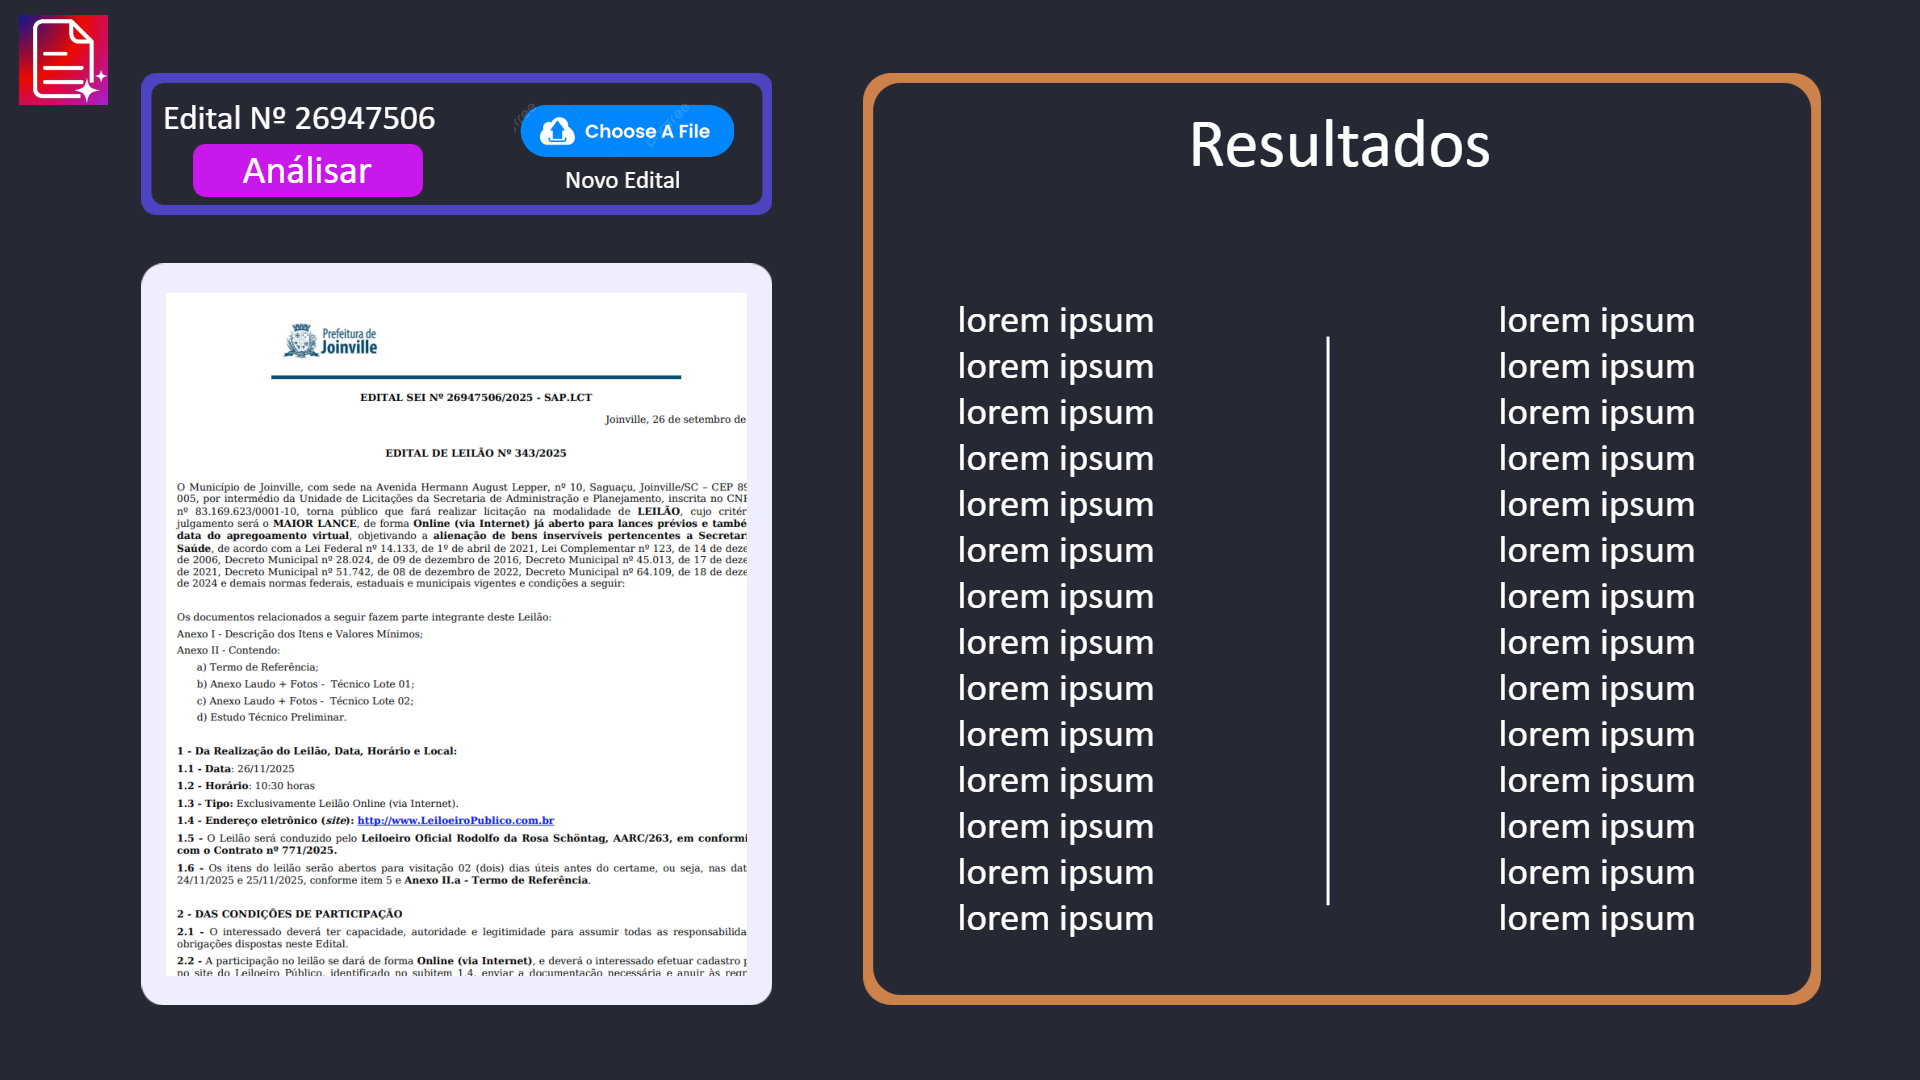
\includegraphics[width=1\textwidth]{figures/agilis-tela.jpg}
  \caption{Tela Principal}
\end{figure}



\subsection{Decisões e Alternativas Consideradas}
A arquitetura híbrida foi escolhida por combinar a eficiência e versatilidade do
Node.js em operações assíncronas com a robustez de bibliotecas Python
voltadas à IA e algoritmos avançados.
Alternativas puramente em Python (Django) foram descartadas devido à menor
integração nativa com outras tecnologias e pela menor versatilidade no
desenvolvimento.

\subsection{Critérios de Escalabilidade, Resiliência e Segurança}
\begin{itemize}
    \item Escalabilidade: sistema rodando em um servidor central, permitindo acesso simples e remoto.
    \item Resiliência: logs e monitoramento de falhas no backend Express.js.
    \item Segurança: hashing de senhas, validação de entrada, autenticação
JWT e observância básica à LGPD.
\end{itemize}


\section{Ferramentas Tecnológicas}

\subsection{Linguagens de Programação}
\begin{itemize}
    \item JavaScript pela sua versatilidade, facilidade de desenvolvimento e
integração com outras tecnologias.
    \item Python pela sua robustez e versatilidade no desenvolvimento de
algorítimos complexos e modelos de IA.
\end{itemize}

\subsection{Frameworks e Bibliotecas}
\begin{itemize}
    \item Express.js pela versatilidade e velocidade no desenvolvimento web, além
da ótima performance.
    \item FastAPI pela versatilidade e velocidade no desenvolvimento de APIs
Python, além da ótima performance.
    \item Pandas pela facilidade de uso e altíssima compatibilidade com outras
bibliotecas e algorítimos Python.
    \item Também serão utilizadas outras bibliotecas variadas a serem decididas
ao longo do desenvolvimento, sendo elas bibliotecas de interfaces visuais e
algorítmos.
\end{itemize}

\subsection{Ferramentas de Desenvolvimento e Gestão}
\begin{itemize}
    \item Visual Studio Code
    \item GitHub
\end{itemize}

\section{Considerações de Segurança}
As principais ameaças são injeção de código malicioso em uploads,
roubos de credenciais, falhas de autenticação e reprocessamento indevido de
arquivos duplicados.

\subsection{Medidas de Mitigação}
\begin{itemize}
    \item Hashing e criptografia de senhas;
    \item Validação rigorosa dos dados de entrada;
    \item Controle de acesso baseado em tokens JWT;
    \item Limitação de tamanho e formato dos uploads.
\end{itemize}

\subsection{Normas e Boas Práticas Seguidas}
\begin{itemize}
    \item LGPD — proteção e confidencialidade de dados de login;
\end{itemize}

\subsection{Responsabilidade Ética}
Embora o sistema utilize IA, ele opera exclusivamente sobre documentos
públicos e não processa dados pessoais sensíveis, mantendo aderência aos
princípios éticos de uso responsável de inteligência artificial.

\subsection{Conformidade e Normas Aplicáveis}
O projeto está em conformidade com:
\begin{itemize}
    \item Lei nº 13.709/2018 (LGPD) — aplicável à gestão de contas de
usuários e autenticação;
\end{itemize}

% -----------------------------------------------------------------
% PRÓXIMOS PASSOS
% -----------------------------------------------------------------
\section{Próximos Passos}
\begin{itemize}
  \item Definição dos algoritimos de IA que serão utilizados.
\end{itemize}

\newpage
\addcontentsline{toc}{section}{Referências}

\begin{thebibliography}{99}
\bibitem{lgpd} LGPD. Lei nº 13.709/2018. Disponível em: \url{https://www.gov.br/cidadania/pt-br/acesso-a-informacao/lgpd}.
\end{thebibliography}

\newpage

\section{APÊNDICE A - TÍTULO}
Um apêndice é um elemento complementar de um trabalho acadêmico
que contém materiais produzidos pelo próprio autor e que ajudam a esclarecer
ou detalhar informações do corpo do texto sem interromper o fluxo da leitura.
Podem ser incluídos, por exemplo, questionários ou formulários utilizados
na pesquisa, códigos-fonte de programas, tabelas extensas, gráficos detalhados,
dados brutos, documentações técnicas, instruções de uso de protótipos,
descrições de experimentos ou procedimentos metodológicos.
Além de quaisquer outros materiais que sejam relevantes para a
compreensão do trabalho, mas que seriam excessivamente longos ou técnicos
se colocados no corpo principal do texto.

\section{ANEXO A - TÍTULO}
Um anexo é um elemento complementar de um trabalho acadêmico que
contém materiais provenientes de fontes externas ao autor, utilizados para
fornecer informações adicionais ou fundamentar o estudo, sem alterar o
conteúdo principal do trabalho.
Podem ser incluídos, por exemplo, normas técnicas, manuais, relatórios
de terceiros, gráficos ou tabelas publicadas, legislações, documentos oficiais ou
quaisquer outros materiais de referência que sejam relevantes para a
compreensão ou validação do projeto, mas que não foram produzidos pelo
próprio autor.

\newpage

\begin{center}
\Large\bfseries BANCA EXAMINADORA
\end{center}

\vspace{2.8cm}

\begin{center}
\normalsize
Nome do Orientador e Titulação\\
Católica de Santa Catarina
\end{center}

\vspace{2.2cm}

\noindent\textbf{Membros:}

\vspace{1.6cm}

\begin{center}
Nome e Titulação\\
Católica de Santa Catarina
\end{center}

\vspace{1.9cm}

\begin{center}
Nome e Titulação\\
Católica de Santa Catarina
\end{center}

\vspace{1.9cm}

\begin{center}
Nome e Titulação\\
Católica de Santa Catarina
\end{center}


\newpage
\section*{Avaliações dos Professores}
\vspace{1cm}
\textbf{Considerações Professor/a:} \\[0.3cm]
\rule{\textwidth}{0.5pt}\\[0.5cm]
\rule{\textwidth}{0.5pt}\\[0.5cm]
\rule{\textwidth}{0.5pt}\\[0.5cm]
\rule{\textwidth}{0.5pt}\\[0.5cm]
\rule{\textwidth}{0.5pt}\\[0.5cm]
\rule{\textwidth}{0.5pt}\\[0.5cm]
\rule{\textwidth}{0.5pt}\\[0.5cm]
\rule{\textwidth}{0.5pt}\\[0.5cm]
\rule{\textwidth}{0.5pt}\\[0.5cm]
\rule{\textwidth}{0.5pt}\\[0.5cm]
\rule{\textwidth}{0.5pt}\\[0.5cm]
\rule{\textwidth}{0.5pt}\\[0.5cm]
\rule{\textwidth}{0.5pt}\\[0.5cm]
\rule{\textwidth}{0.5pt}\\[0.5cm]
\rule{\textwidth}{0.5pt}\\[0.5cm]
\rule{\textwidth}{0.5pt}\\[0.5cm]
\rule{\textwidth}{0.5pt}\\[0.5cm]
\rule{\textwidth}{0.5pt}\\[0.5cm]
\rule{\textwidth}{0.5pt}\\[0.5cm]
\rule{\textwidth}{0.5pt}\\[0.5cm]
\rule{\textwidth}{0.5pt}\\[0.5cm]

\end{document}